\documentclass{article}

%%PACKAGES%%
\usepackage{datetime}
\usepackage[UKenglish]{isodate}
\usepackage{hyperref}
\usepackage{graphicx}

\begin{document}

%%%%%%%%%%%%%%%%%%%%%%%%%%%%%%%%%%%%%%%%%%%%%%%%%%%%%%%%%%%%%
\begin{titlepage}
	\centering
	{\scshape\LARGE Royal Institute of Technology \par}
    {\scshape\LARGE KTH \par}
	\vspace{2cm}
	{\scshape\Large Master Thesis Report \par}
	\vspace{1.5cm}
	{\huge\bfseries IP over Bluetooth Low Energy in the Contiki OS
 \par}
	\vspace{3cm}
    {\Large\itshape By:\par}
    \vspace{1cm}
	{\Large\itshape Johan Gasslander\par}
	\vfill
% Bottom of the page
\cleanlookdateon
	{\large \today}
\end{titlepage}

\pagenumbering{roman}
%%%%%%%%%%%%%%%%%%%%%%%%%%%%%%%%%%%%%%%%%%%%%%%%%%%%%%%%%%%%%
\section*{Abstract}
Bluetooth low energy (BLE) has since its inclusion in Bluetooth v4.0 standard emerged as a contender for weaving sensors and other devices into the fast developing Internet of Things. Using low power IP features is an essential part of an efficient IoT. The BLE and 6LoWPAN provide such features and have been emerging in technologies.\\
Contiki is a tiny, low-power, operating system with built in support for the 6LoWPAN standard and other networking protocols. In this thesis, a port for Contiki to the nRF52 is evaluated with two applications utilizing IP over BLE on the nRF52832 SoC.
\newpage

%%%%%%%%%%%%%%%%%%%%%%%%%%%%%%%%%%%%%%%%%%%%%%%%%%%%%%%%%%%%%
\section*{List of abbreviations} 
\begin{itemize}
\item 
BLE - Bluetooth Low Energy or Bluetooth Smart
\item 
IPv6	 - Internet Protocol version 6
\item 
GATT - Generic Attribute Profile
\item 
GAP - Generic Access Profile
\item 
CoAP - Constrained Application Protocol
\item 
RPL - Routing Protocol for Low-power and lossy networks
\item 
SICS - Swedish Institute of Computer Science
\item 
IoT - Internet of Things
\item 
6LoWPAN - IPv6 over Low-power Personal Area Network
\item 
MAC - Media Access Protocol
\item 
MCU - Microcontroller Unit
\end{itemize}
\newpage

%%%%%%%%%%%%%%%%%%%%%%%%%%%%%%%%%%%%%%%%%%%%%%%%%%%%%%%%%%%%%
\tableofcontents
\newpage 

\pagenumbering{arabic}
%%%%%%%%%%%%%%%%%%%%%%%%%%%%%%%%%%%%%%%%%%%%%%%%%%%%%%%%%%%%%
\section{Background}
Since Bluetooth low energy (BLE) was included in the Bluetooth v4.0 standard in 2010, it has emerged as a strong contender in the fast developing Internet of Things. In particular, small devices and weaving sensors have been utilizing BLE. Part of BLEs quick entry can be subscribed to its natural, tight integration with classic Bluetooth within the same protocol stack. Bluetooth classic’s existing presence in PC’s and smartphones promote manufacturers to opt for BLE in favor of rival technologies, when considering connectivity and networking options to link products to the IoT.\\
The momentum for BLE-connected IoT is gathering, with the recent introduction of the Low-power IP feature, via the Internet Protocol Support Profile (IPSP), to Bluetooth v4.2. This feature paves the way for direct IPv6/6LoWPAN connections between the devices and the Internet. Nordic Semiconductor’s nRF51 and nRF52 series provide a proprietary, free-of-charge BLE protocol stack, in the form of a precompiled and linked firmware library.\\
The API usually lies around the Generic Attribute Profile (GATT) layer, above which application-specific profiles, e.g., a weight scale profile with weight scale and body composition services, are implemented by the application developer.\\
Low power systems are an important piece of the IoT. The open source project Contiki OS has been the choice of many IoT projects due to its compact, high-quality IPv6/6LoWPAN stack, which can be used with IoT routing protocol RPL and application-layer protocols CoAP and MQTT. Below the network layer, the dominant radio technology used by Contiki platforms is the PHY layer of the open standard IEEE 802.15.4 which is the combined with a rich set of MAC protocols.\\
\subsection{Technical background}
\subsubsection{Contiki}
Contiki is a lightweight operating systems designed for embedded systems and sensor networks. Contiki is officially supported for a number of platforms such as the SkyMote, Z1, AVR-Raven, C64, CC2530dk and now nRF52dk. Pre-built application implementations such as CoAP, DHCP, FTP, MQTT and shell are included to ease development.
In order to save power, Contiki uses ContikiMAC - a radio duty cycle media access control protocol which utilizes principles behind low-power listening while increasing power efficiency.

\subsubsection{Proto threads}
Protothreads in the Contiki system are software based threads written in C. The threads are aimed for extremely low memory constrained systems and can be used with or without an RTOS. \cite{proto} Proto threads are particularly efficient at running linear code while also saving memory by omitting thread stacks. All threads share a stack and context switching rewinds the stack. Local variables are therefore not preserved between between blocks and must be preserved or regarded as volatile.
Blocking calls in nested functions are made by spawning new proto threads.


\subsubsection{BLE}
Bluetooth Low Energy (or Bluetooth Smart) was introduced as Wibree by Nokia in 2006 \cite{wibree} and merged into the main Bluetooth standard in 2010 when the Bluetooth Core Specification Version 4.0 was adopted. It is defined as a WPAN (Wireless Personal Area Network) meaning it is designed to work on short range personal devices such as heart rate monitors, smart watches and insulin dispensers. The current version supports a myriad of application profiles for similar devices by default.

\subsubsection{GATT}
The Attribute Profiles defines rules how data is accessed from a peer device.\cite{blehandbook} Data stored within an attribute server which an attribute client can read and write. Clients send queries to the server and receives response messages which it can use to read/write any attribute on the server.\\
The protocol defines six types of messages: requests from client to server, responses from server for a request from client, commands without response from the client, notifications from the server to the client without response, indications from server to client and responses from client to indications from server.\\
Each attribute has a unique handle id to separate attributes, a type to identify the data and a value for the data. Attributes can require authentication as defined by the protocol. These requirements can not be discovered without an error in response to an attempt to access the attribute.\\
In the layer above the attribute profile lies the Generic Attribute Profile which defines the types of attributes and how they are used. One profile may contain one or many services. Services are divided into primary and secondary services. Primary services can contain secondary services that are used by the primaries. Services consist of one or more characteristics which have properties to the value, a single value and one or more descriptors. In \pageref{fig:gatt} we see the structure of a profile and its constitution.\\

%%%\fig{1}

\begin{figure}[p]
	\centering
	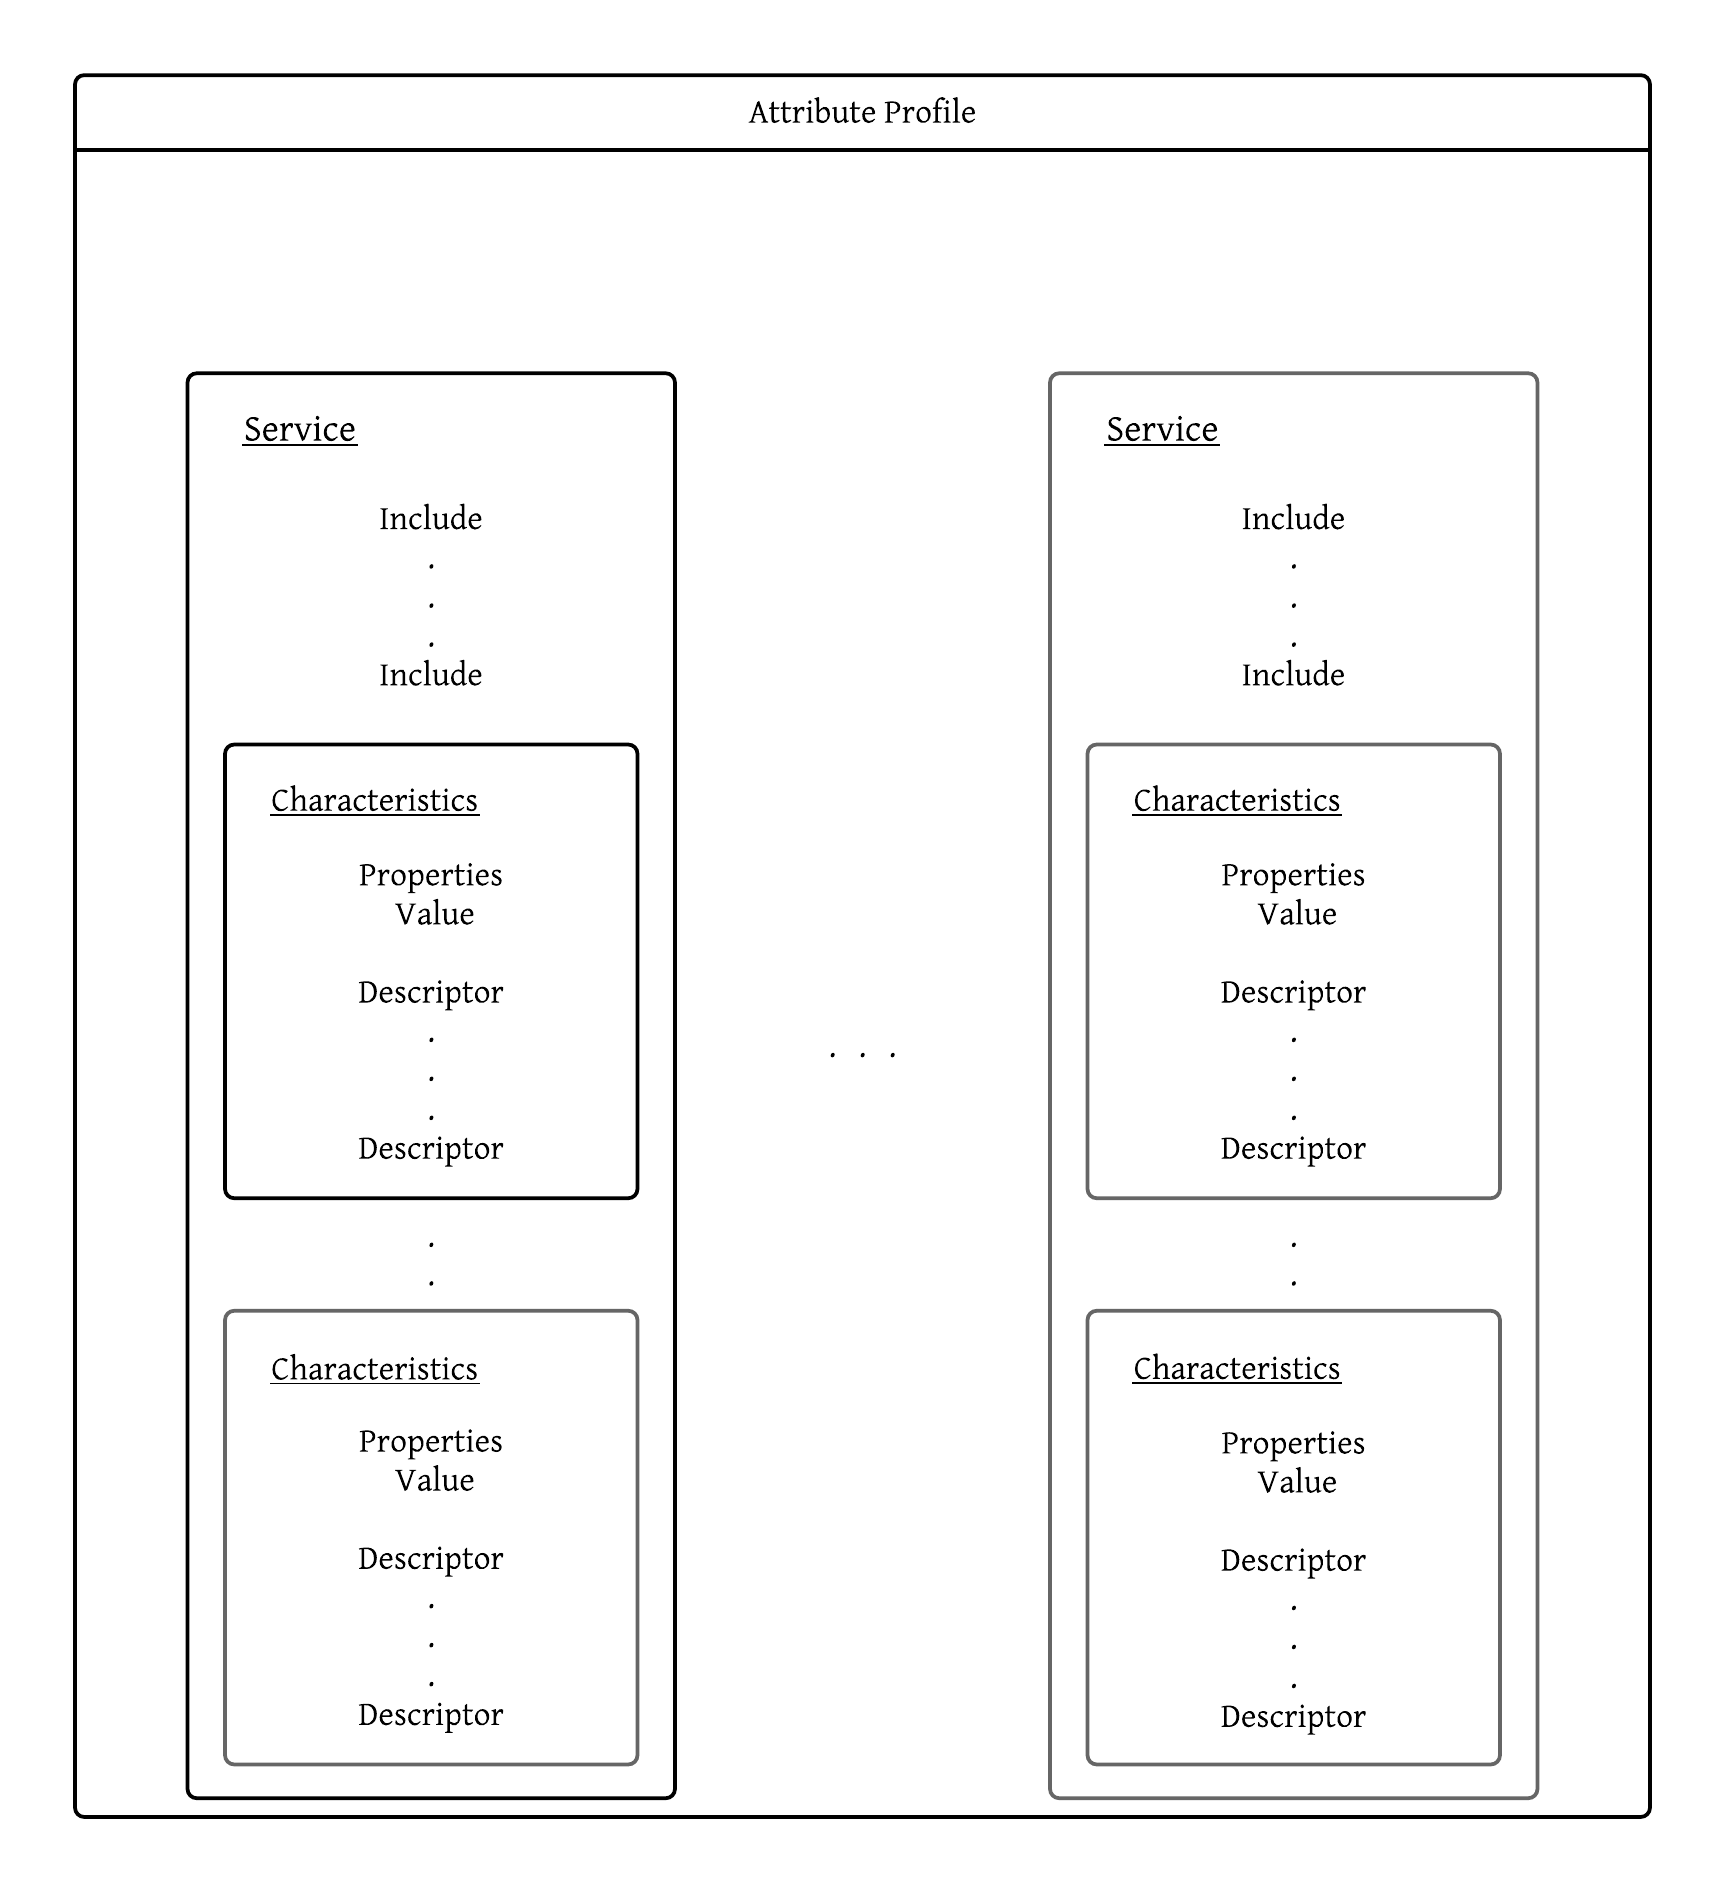
\includegraphics[scale=0.2]{gatt}
	\caption{GATT}
    \label{fig:gatt}
\end{figure}

The Application layer, above the GATT, defines specifications for the attribute groups defined in GATT.

\subsubsection{GAP}
In order to maintain the connection to services, the Generic Access Profile defines how the to discover, connect and bond to, devices. The layer also enables privacy by using resolvable private addresses which are constantly changed while advertising in order to avoid being identified. In order to be able to connect to devices that seeks privacy, the GAP specifies how to resolve the private addresses and how to connect.

Connecting through general connection establishment in GAP could cost more energy from the node since it must transmit more packages during connection than during auto-connection procedure. auto-bonding does however require a bond to be established

\subsubsection{IPSP}
Internet Protocol Support Profile enables BLE to send IPv6 packets over BLE transport and is compatible with Bluetooth core specification v4.1 and above.\cite{bleipsp} 
IPSP defines two roles: node and router. The router node is used for devices that can route IPv6 packets. The node role is for any device which may originate application packets or any node that consume application packets. Also, the node contains the IPSS (Internet Protocol Support Service) which uses GATT to allow discovery of the node. Devices can use both roles if they can both route and need to handle packets.

\subsubsection{6LoWPAN}
IPv6 over low power personal area networks utilises encapsulation and header compression mechanisms to send IPv6 packets through IEEE 802.15.4 networks. IEEE 802.15.4 is a standard which specifies the physical layer and the media access control. Developed by the 6LoWPAN IETF group.

\subsubsection{nRF52832}
The nRF52832 SoC from Nordic Semiconductors provides hardware features such as a 2.4GHz radio, supporting Bluetooth Smart, ANT and proprietary RF (i.e Gazel).
The system features 512 kB flash memory and 64 kB RAM, the 32-bit ARM Cortex-M4F MCU, configurable analogue and digital I/O mapping, GPIO, 3 master/slave SPI, 2 I2C, AES hardware encryption and automatic power management.\cite{nrf52832}\\
The hardware supplied for this thesis is two nRF52 Preview DK boards. This DK supplies all RF features, 4 LEDs, 4 hardware buttons, coin-cell battery holder, micro USB connector for power supply and flashing capabilities, pins for measuring power consumption, port for external programming/debugging,  Arduino Uno Rev. 3 compatible connector for use with 3rd party shields and an NFC antenna.\\

The software architecture features a separation between the SoC and the application layer called SoftDevice. The SoftDevice can be chosen to supply a set of features and ensures that applications can be coded and debugged independently of the protocol stack, reducing development efforts and bugs and their complexity.\\

\subsection{Nordic Semiconductor Smartphone Apps}
Nordic Semiconductors supply a series of Android applications designed to test the nRF series both with and without example applications attached.
The nRF Master Control Panel shows available BLE connections and supports bonding. It also provides a view of services on the devices, their parameters and descriptors.
the nRF Toolbox provides a series of applications to test example software provided by Nordic Semiconductors. The applications utilize standard Bluetooth services such as heart rate monitors, blood pressure monitors and proximity sensors.\\

\subsection{Summary}
The tools and technologies listed above are used together in order to build small constrained devices that interface with regular infrastructure, enabling them to communicate and perform new tasks in a power and cost effective manner.

\section{Introduction}
In order for the newly released nRF52dk to be used with Contiki, a port has been made by Nordic Semiconductors. When the project started it was on pull request and as of the 1st of June, the port is part of the master branch of Contiki. \cite{upstream}
This port needs evaluation to see if it is working correctly and what services and functionalities work as expected and follow performance needs.\\

%%%%%%%%%%%%%%%%%%%%%%%%%%%%%%%%%%%%%%%%%%%%%%%%%%%%%%%%%%%%%
\section{Purpose}
In order to know if the nRF52 port made by Nordic Semiconductors is efficient and useful, a series of programs will be made to evaluate the port and platform combination.\\

\section{The Contiki port}
The Contiki port for the nRF52 development kit preview version is made and maintained by Bober Wojciech at Nordic Semiconductors. \cite{port}
The port includes support for the boards buttons, LEDs, system clock and timers, UART, Watchdog, hardware RNG, RTT I/O, temperature sensor, IPV6 and the slave mode for BLE. The port does not include the BLE master mode which means that communication between two nodes needs to happen through IPv6 traffic through a routing device using the IPSP for BLE. It does not support the IPv4 network stack.\\
It is designed around the nRF5 IoT SDK which is required to compile all parts. The SDK also supplies the $s1xx-iot-prototype3_nrf52$ SoftDevice.
The port support the two DKs, PCA10040 and PCA10036. For this thesis, the nRF52dk boards utilize, PCA10040.



%%%%%%%%%%%%%%%%%%%%%%%%%%%%%%%%%%%%%%%%%%%%%%%%%%%%%%%%%%%%%
\section{Method}
\subsection{Process}
Half the time was spent on gathering data and on experimenting to learn the platform and relevant technologies. %%Crude
Now its most of the time.

Tasks
\begin{itemize}
\item
Several small applications are built to explore the port and to setup the toolchain properly
\item
An application will be implemented that use BLE to transmit IP packets
using IPSP. The applications use the Contiki Erbium engine to transmit CoAP packets.
\item
Evaluate the application implementation and find flaws and strengths
\item
Suggest improvements to the port and future work on the board. Applications and usability.
\end{itemize}


\subsection{Optimizations}
Performance optimization will be measured on speed of transmission and memory footprint.

%%%%%%%%%%%%%%%%%%%%%%%%%%%%%%%%%%%%%%%%%%%%%%%%%%%%%%%%%%%%%
\section{Application implementation}
The implementations will consist of two version of a model of a code lock. The nodes will be a certification agent and one or more access points(keypads controlling a door.) Two implementations will be made, one with DLTS and one without.
Performance testing is done primarily on throughput.\\

Using tinyDTLS \cite{tinydtls} to introduce an option in the erbium engine in Contiki, we should be able to see that a secure communication can be used with CoAP.


Master role
The master role in IPSP is needed for a nRF52dk device to find and connect to another device. The role is a part of the official IPSP specification and requires the node to scan for advertisements, process them and connect. The already existing ble-core.c and ble-mac.c in the port are extended with the required iterfacing to the Firmware which does the actual scanning and connecting. The ble-mac is the media access protocol that is the default for the port set in the contiki-conf.h in the platform specific code for contiki. This means that contiki will use this interface medium to establish all links through radio transmission.

the required functionalities for the ble-core and mac are as follows
Start scanning
Parsing scanned data
Since there is already code for the node role. The code must be modified to ensure the existing functionality is not impaired.


ISSUES
the softdevice is halted at $m_ble_evt_buffer_size$\\
The softdevice in slave node is sending the connection response code 0x0004 "LE Result: Connection Refused - No Resources Available"\\
0000   0e 00 05 00 15 03 0a 00 00 00 00 00 00 00 00 \textbf{00}  ................\\
0010  \textbf{04} 00                                             ..\\
What is error 4? MAC_TX_ERR?\\
RTT VS VCOM which is super slow\\



\subsection{CoAP}
CoAP Constrained Application Protocol is a way to share data over severely memory and processing constrained networks. This is done by reducing the overhead for each packet and also lowering the payload size. One CoAP message should be able to properly fit into a single IP packet, and datagram, and thus avoids packet fragmentation. \cite{coap}
The implementations use the Erbium CoAP engine which is the CoAP engine for Contiki developed by ETH Zurich and SICS.

\subsection{DTLS}
The transport layer security (TLS) originated DTLS (Datagram TLS) protocol allows client/server applications to communicate in a way that is designed to prevent eavesdropping, tampering, or message forgery. \cite{dtls} The protocol assures equivalent security guarantees. DTLS must be run over a reliable transport channel such as TCP and the protocol can thus not be used to secure unreliable datagram traffic.
For this thesis, the tinyDTLS will be used as it is an open-source implementation which is reduced in overhead to accommodate the constrained environment of the nRF52 board.\\
The DTLS process works as follows: first, a handshake period is initiated where the client sends a request to the server, called ClientHello expecting a HelloVerifyRequest prompting the client to send another ClientHello. The server will then send the ServerHello, along with it's certificate. The client replies with its own certificate and the server responds with a ChangeCipherSpec, indicating the negotiated cipher will now take effect.
The handshake process is protected with RSA and tinyDTLS supports AES-128-CBC for encryption of the sessions and SHA1 for hashing.

In order to establish keys the nodes connect to a bootstrap server which supplies them with login information to a LESHAN server. The LESHAN project is a OMA Lightweight M2M implementation in Java made by the eclipse foundation. \cite{leshan} It supplies libraries for LwM2M client and server applications and its own demo server and client. The server is used by this thesis to supply PSKs for DTLS.

The IOT5 SDK supports TLS and could be used in future works.
%%%%%%%%%%%%%%%%%%%%%%%%%%%%%%%%%%%%%%%%%%%%%%%%%%%%%%%%%%%%%
\section{Results and Discussion}

Board does not handle printout to TTY properly. If too many are called or if they are called from the wrong place (somewhat difficult to replicate these errors) the board system. 
\subsection{Optimizations}
\subsection{Measurements}
\subsection{Analysis}
\subsection{Discussion}

%%%%%%%%%%%%%%%%%%%%%%%%%%%%%%%%%%%%%%%%%%%%%%%%%%%%%%%%%%%%%
\section{Future work}
Fully integrating tinyDTLS into the Contiki OS as a complete feature regardless of platform.\\
Implementing the master role into the port would likely increase the stability and performance of the system due to no longer needing an external routing agent.\\
Tests for the NFC\\
Long time low power operation\\
Compare tinyDTLS to mbedTLS\\
%%%%%%%%%%%%%%%%%%%%%%%%%%%%%%%%%%%%%%%%%%%%%%%%%%%%%%%%%%%%%
\section{Summary}

%%%%%%%%%%%%%%%%%%%%%%%%%%%%%%%%%%%%%%%%%%%%%%%%%%%%%%%%%%%%%
\section{Acknowledgements}
Thanks to B. Wojciech at Nordic Semiconductor, author of the nRF52dk-pr Contiki port, for his support and thanks to everyone at SICS Swedish ICT, especially Shahid Raza and Zhitao He for hosting this thesis project and to Niclas Finne for help on the YanziNetworks tinyDTLS implementation.

\begin{thebibliography}{9}

\bibitem{proto} \url{http://contiki.sourceforge.net/docs/2.6/a01802.html}.
\emph{Contiki 2.6: Protothreads}, fetched 2016/03/15

\bibitem{nrf52832}
\url{http://infocenter.nordicsemi.com/pdf/nRF52832_PS_v1.0.pdf}.
\emph{nRF52832 - Product Specification v1.0}, fetched March 2016

\bibitem{nrf52dk} Nordic Semiconductor,
\emph{nRF52 Preview DK v1.1 product brief}, 2015

\bibitem{wibree} \url{http://company.nokia.com/en/news/press-releases/2006/10/03/nokia-introduces-wibree-technology-as-open-industry-initiative}.
\emph{Wibree from Nokia}, 2006

\bibitem{bluetooth} \url{https://www.bluetooth.com/what-is-bluetooth-technology/bluetooth-technology-basics/low-energy}.
\emph{Bluetooth Smart by Bluetooth}, fetched on 2016/03/15

\bibitem{blehandbook} R. Heydon,
\emph{Bluetooth Low Energy the developer's handbook}, 2013

\bibitem{bleipsp} \url{https://www.bluetooth.org/docman/handlers/DownloadDoc.ashx?doc_id=296307}.
\emph{Internet Protocol Support Profile Bluetooth® Specification}, 2014-Dec-16

\bibitem{RPL} T. Winter, P. Thubert, A. Brandt, J. Hui, R. Kelsey, P. Levis, K. Pister, R. Struik, J. Vasseur, and R. Alexander,
\emph{RPL: IPv6 Routing Protocol for Low-Power and Lossy Networks. RFC 6550}, March 2012

\bibitem{coap} Z. Shelby, K. Hartke, and C. Bormann,
\emph{The Constrained Application Protocol (CoAP). RFC 7252 (Proposed Standard)}, June 2014

\bibitem{erbium} M. Kovatsch, S. Duquennoy, A. Dunkels, 
\emph{A Low-Power CoAP for Contiki}
2011

\bibitem{dtls} E. Rescorla, RTFM, Inc., N. Modadugu, Google, Inc.
\emph{Datagram Transport Layer Security Version 1.2. RFC 6347}, January 2012

\bibitem{port} B. Wojciech,
\url{https://github.com/wbober/contiki/tree/nrf52dk-pr}
\emph{Contiki for nRF52 Development Kit}, fetched May 2016

\bibitem{tinydtls} 
\url{https://projects.eclipse.org/projects/iot.tinydtls}
\emph{tinyDTLS}, fetched May 2016

\bibitem{leshan} eclipse Foundation
\url{https://github.com/eclipse/leshan}
\emph{LESHAN}, fetched June 2016

\bibitem{upstream}
\url{https://github.com/contiki-os/contiki/pull/1469}
\emph{the nrf52dk port merged to the Contiki master}, fetched June 2016

\end{thebibliography}
\newpage

%%%%%%%%%%%%%%%%%%%%%%%%%%%%%%%%%%%%%%%%%%%%%%%%%%%%%%%%%%%%%
\appendix
\section{Aasdasd}
\end{document}